\-Copyright (\-C) 2012 by \-Fabian \-Deitelhoff $<$\href{mailto:FH@FabianDeitelhoff.de}{\tt \-F\-H@\-Fabian\-Deitelhoff.\-de}$>$ and \-Christof \-Geisler $<$\href{mailto:christof.geisler@stud.fh-swf.de}{\tt christof.\-geisler@stud.\-fh-\/swf.\-de}$>$

\-Solar\-System\-Simulation is free software\-: you can redistribute it and/or modify it under the terms of the \-G\-N\-U \-General \-Public \-License as published by the \-Free \-Software \-Foundation, either version 3 of the \-License, or (at your option) any later version.

\-Solar\-System\-Simulation is distributed in the hope that it will be useful, but \-W\-I\-T\-H\-O\-U\-T \-A\-N\-Y \-W\-A\-R\-R\-A\-N\-T\-Y; without even the implied warranty of \-M\-E\-R\-C\-H\-A\-N\-T\-A\-B\-I\-L\-I\-T\-Y or \-F\-I\-T\-N\-E\-S\-S \-F\-O\-R \-A \-P\-A\-R\-T\-I\-C\-U\-L\-A\-R \-P\-U\-R\-P\-O\-S\-E. \-See the \-G\-N\-U \-General \-Public \-License for more details.

\-You should have received a copy of the \-G\-N\-U \-General \-Public \-License along with \-Solar\-System\-Simulation. \-If not, see $<$\href{http://www.gnu.org/licenses/}{\tt http\-://www.\-gnu.\-org/licenses/}$>$.

\begin{DoxyAuthor}{\-Author}
\-Fabian \-Deitelhoff $<$\href{mailto:FH@FabianDeitelhoff.de}{\tt \-F\-H@\-Fabian\-Deitelhoff.\-de}$>$ 

\-Christof \-Geisler $<$\href{mailto:christof.geisler@stud.fh-swf.de}{\tt christof.\-geisler@stud.\-fh-\/swf.\-de}$>$
\end{DoxyAuthor}
\-Circumference of an ellipse according to \-Ramanujan\-:

\[ u \approx (a + b) \cdot \pi \cdot ( 1 + \frac{ 3 \lambda^2}{10 + \sqrt{4 - 3 \lambda^2}}) \quad \hspace{0.5cm} with \hspace{0.5cm} \quad \lambda = \frac{a-b}{a+b} \]

 
\begin{DoxyImage}
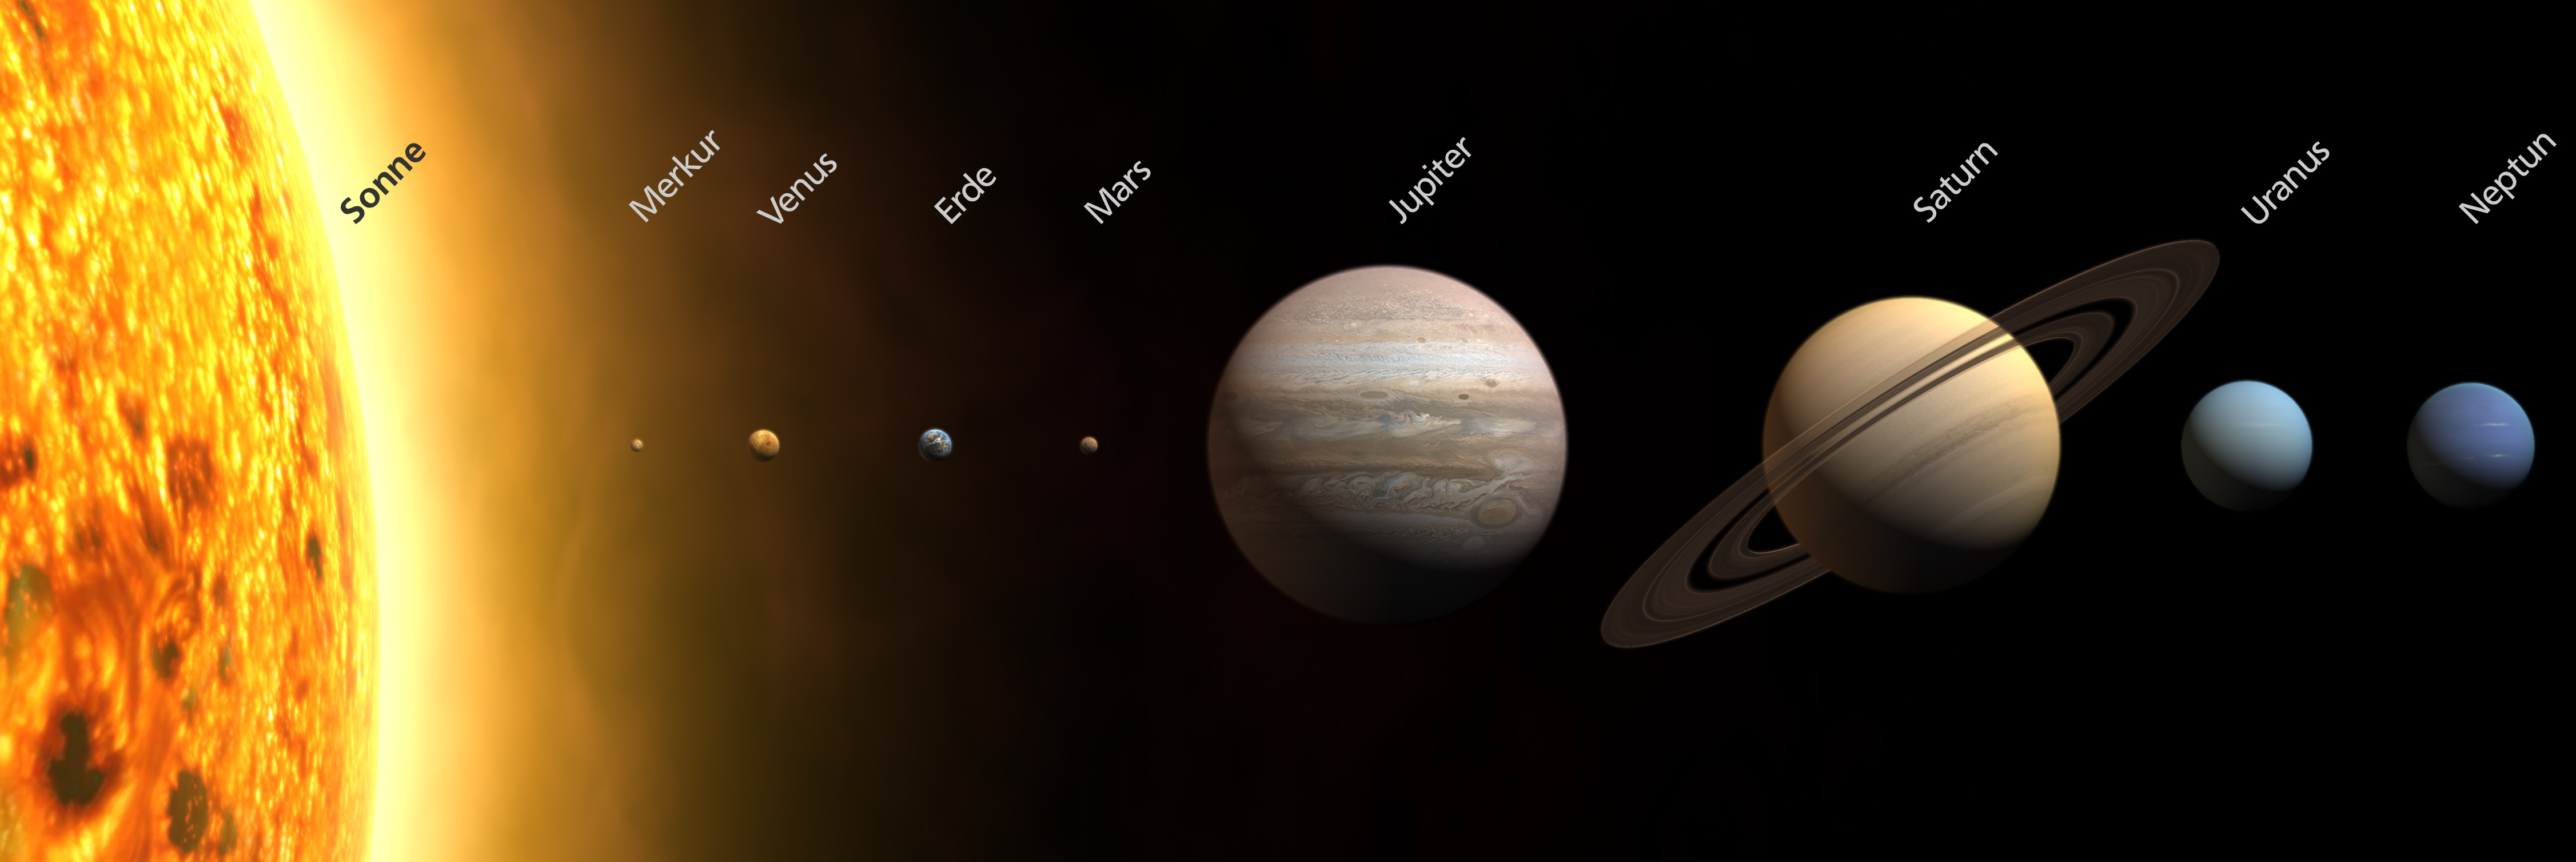
\includegraphics[width=12cm]{about.jpg}
\caption{\-Planets of our solar system}
\end{DoxyImage}
 